\subsection{Location Providers}

A device may have several providers. Location can be obtained directly from satellites 
(GPS). Or can be derived from Wi-fi access points information, mobile communication tower's location. 

The devices are condensed in the provider: GPS\_PROVIDER ("gps"), NETWORK\_PROVIDER ("network").
Also usually exists a PASSIVE\_PROVIDER (another app) 

GPS is accurate, has more info, more power consumption, more delay,
needs line of sight to satellites (weak signals). 

Network is less accurate, has less consumption, less delay, interiors.

Android manifest must declare permissions:

\begin{itemize}
    \item ACCESS\_COURSE\_LOCATION
    \item ACCESS\_FINE\_LOCATION
\end{itemize}

\begin{figure}[h]
\centering
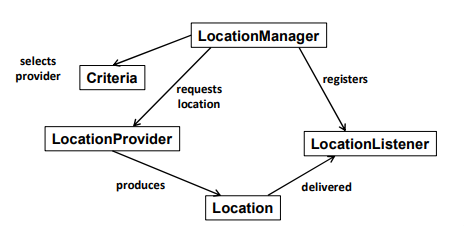
\includegraphics[width=0.9\linewidth]{figures/07_location_manager_diagram.png}
\caption{Location Manager Diagram}
\label{fig:location_manager_diagram}
\end{figure}


\subsection{LocationListener} 
Interface declaring methods (callbacks) where information is delivered
after requesting a location. 

\begin{lstlisting}[title=LocationListener interface]
public interface LocationListener {
    void onLocationChanged(Location location);
    void onProviderDisabled(String provider);
    void onProviderEnabled(String provider);
    // Not called in api 29.
    // status: OUT_OF_SERVICE, TEMPORARILY_UNAVAILABLE,AVAILABLE
    // satelities: nr. of satelities in gps. 
    void onStatusChanged(String provider, int status, Bundle extras);
}
\end{lstlisting}

\subsection{LocationManager}

System service for requesting locations and selecting a provider. 
Obtained in an Activity: 

\begin{lstlisting}
locationManager = (LocationManager) getSystemService(LOCATION_SERVICE);
\end{lstlisting}

Locations should be requested only when the activity is active and cancelled 
when it stops being in foreground.
So requests can be done in the \texttt{onResume()} callbackof the activity, 
from the LocationManager object, with:

\begin{lstlisting}
// minTime: minimum time or distance for a new location
// criteria: selection of a provider 
// listener: class implementing the listener
// looper: null for the current thread
requestLocationUpdates(long minTime, float minDistance, Criteria criteria,LocationListener listener, Looper looper); 
\end{lstlisting}

In \texttt{onPause()} we should cancel the request and stop the provider:

\begin{lstlisting}
removeUpdates(LocationListener listener) 
\end{lstlisting}


It is also possible to request a single location or an alert of proximity to agiven location expressed in latitude or longitude.
\texttt{requestSingleUpdate(...) and addProximityAlert(...)}. 

\subsection{Location}
Locations are delivered to LocationListener 

\begin{itemize}
    \item They bring latitude and longitude;
    \item The provider that has generated it;
    \item The time it was generated;

\end{itemize} 

If the provider have the information, it can also contain: 
\begin{itemize}
    \item The altitude of the location;
    \item The accuracy of the location;  
    \item The bearing if the device is moving
    \item The speed also if it is moving
    \item The number of satellites used to obtain the location
\end{itemize} 

Some convenience methods allow: 
\begin{itemize}
    \item To know the bearing from this location to another (geodesic)
    \item The distance between locations (along a geodesic)
    \item Obtain a convenient String representation
\end{itemize}

\begin{figure}[h]
\centering
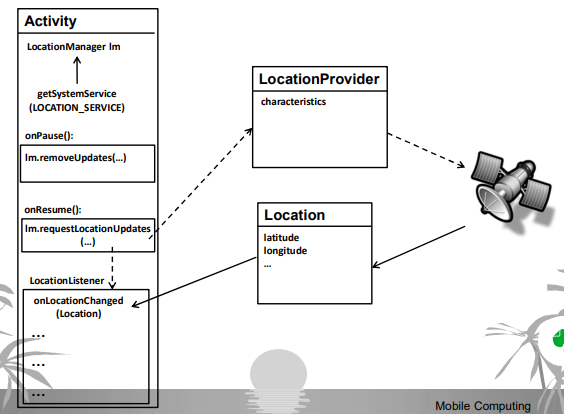
\includegraphics[width=0.8\linewidth]{figures/07_receiving_location_information.png}
\caption{Receiving location information}
\label{fig:receiving_location_information}
\end{figure}

\subsection{Sensors}
Android has support for several sensors and a common API to get their measurements.
Sensors available include:
\begin{itemize}
    \item  movement sensors; 
    \item  orientation sensors;
    \item  environment sensors;
\end{itemize} 

Sensors can be divided into: 
\begin{itemize}
    \item physical sensors giving actual measurements of some quantity;
    \item synthesized sensors fusing and processing the measurements of other physical sensors to calculate another quantity;
\end{itemize}

Sensors can be characterized by:
\begin{itemize}
    \item Range and resolution (minimum, maximum and step value);
    \item Rate of measurement (nr. of measurements per time unit);
    \item Power consumption;
\end{itemize}

\subsubsection{Sensor type supported}

Android defines a constant for each of the 
sensor types supported bythe operating system, in the Sensor class. 
But each device may haveonly a few of those sensors.

\begin{lstlisting}[title=physical types]
movement:
    TYPE_ACCELEROMETER (3D)
    TYPE_GYROSCOPE (3D)
orientation:
    TYPE_MAGNETIC_FIELD (3D)
environment:
    TYPE_AMBIENT_TEMPERATURE
    TYPE_LIGHT
    TYPE_PRESSURE
    TYPE_PROXIMITY
    TYPE_RELATIVE_HUMIDITY
\end{lstlisting} 

\begin{lstlisting}[title=synthetized types]
TYPE_GRAVITY (3D)
TYPE_LINEAR_ACCELERATION (3D)
TYPE_ORIENTATION (3D)
TYPE_ROTATION_VECTOR (3 or 4D)
TYPE_SIGNIFICANT_MOTION (Trigger)
\end{lstlisting}

\subsubsection{Sensor on a device}
It's possible for a device to have more than one sensor of the same type.
It's uncommon for physical sensors, but can happen with synthesized
sensors (more than one implementation). 

When an application requests the sensors
of a certain type (with \texttt{getSensorList(type)}),
the system returns an array of sensors. 


The \texttt{SensorManager} is the starting point and can be obtained from
the \texttt{Activity} with:

\begin{figure}[h]
\centering
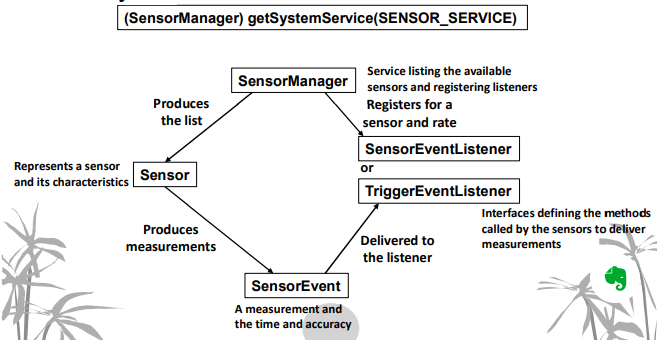
\includegraphics[width=0.8\linewidth]{figures/07_sensor_api_classes.png}
\caption{Sensor API classes}
\label{fig:sensor_api_classes}
\end{figure}

\subsubsection{Movement and Orientation}
Movement quantities are presented in the device coordinate system.
Orientation measures are in the earth coordinate system (except
\texttt{TYPE\_ORIENTATION} and \texttt{getOrientation()} measurements).

\texttt{TYPE\_ORIENTATION} and \texttt{getOrientation()} measurements earth coordinate system.

\begin{figure}[h]
\centering
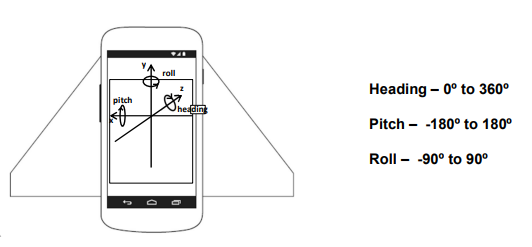
\includegraphics[width=0.8\linewidth]{figures/07_orientation_measurements.png}
\caption{Orientation measurements}
\label{fig:orientation_measurements}
\end{figure}

\subsubsection{SensorManager}

Activities get it from the system and it knows the sensors available on the device.
We can get a list of all or of a single type of sensors and it's possible to have more than one sensor of a given type
(specially of fusion/synthesized sensors). 

It can register the \texttt{SensorEventListener} for one or
more sensors. 
It defines some measure transformation methods: 
\begin{itemize}
    \item \texttt{getRotationMatrixFromVector()} uses the \texttt{ROTATION\_VECTOR} 
sensor and computes a rotation matrix;
    \item \texttt{getRotationMatrix()}: computes Inclination and Rotation matrices from gravity and
geomagnetic fields
\item \texttt{getInclination()} (from the Inclination matrix)
\item \texttt{getOrientation()} (from the Rotation matrix)
\item \texttt{getAltitude()}  From the atmospheric pressure here and at sea level

\end{itemize}

\subsubsection{SensorEventListener}
Interface declaring methods (callbacks) where measurements are
delivered after registering it for a sensor.
Measurements are represented by an instance of \texttt{SensorEvent}. 

\begin{lstlisting}
public interface SensorEventListener {
    // The event has sensor, values[], timestamp, accuracy
    void onSensorChanged(SensorEvent event);
    void onAccuracyChanged(Sensor sensor, int accuracy);
}

// The accuracy can be one of SENSOR_STATUS_ACCURACY_HIGH, SENSOR_STATUS_ACCURARY_MEDIUM,
// SENSOR_STATUS_ACCURACY_LOW, SENSOR_STATUS_ACCURARY_UNRELIABLE. 

// For sensors producing an event at a time (like the SIGNIFICANT_MOTION detector)
// use the abstract class:
public abstract class TriggerEventListener {
    public void onTrigger(TriggerEvent event);
}
\end{lstlisting}  

\begin{figure}[h]
\centering
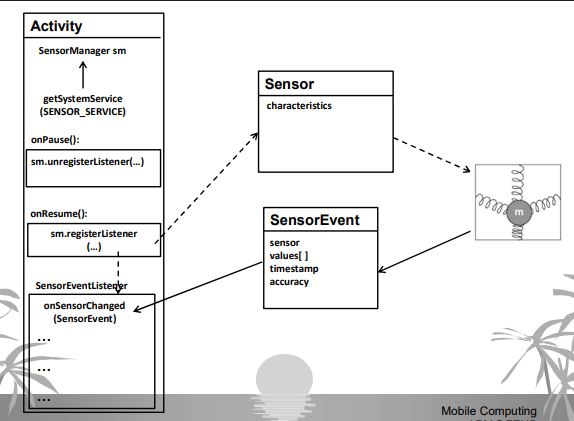
\includegraphics[width=0.8\linewidth]{figures/07_receiving_sensor_measurement.png}
\caption{Receiving sensor measurement}
\label{fig:receiving sensor measurement}
\end{figure}

\subsection{Noise and signal processing}

Many sensors produce several kinds of noise:
\begin{itemize}
    \item High frequency variations with significant amplitudes 
    \item Low frequency deviations (drifts)
\end{itemize} 

Some simple frequency domain filters are useful:

\begin{itemize}
    \item \textbf{Low pass filters}: Weighted smoothing, simple moving average,
simple moving median;
    \item \textbf{High pass filters}: inverse low pass filter;
    \item \textbf{Band pass filters}: Simultaneous low and high pass;
    \item Kalman filters
\end{itemize}





